\section{Square lattice}
\label{sec:square}

The case of the square lattice is extensively studied both at the mean field level and using \acs{QMC}.
Mean field results suggest that at half filling,  antiferromagnetic order persists even at weak coupling \cite{claveau_mean-field_2014, gouveia_magnetic_2015}, a result that we confirm with \acs{QMC}, reproducing the results of \cite{white_numerical_1989, hirsch_two-dimensional_1985}.

\begin{figure}[H]\label{fig:mfHubbardPhaseDiagram}
\hspace{0.68cm}
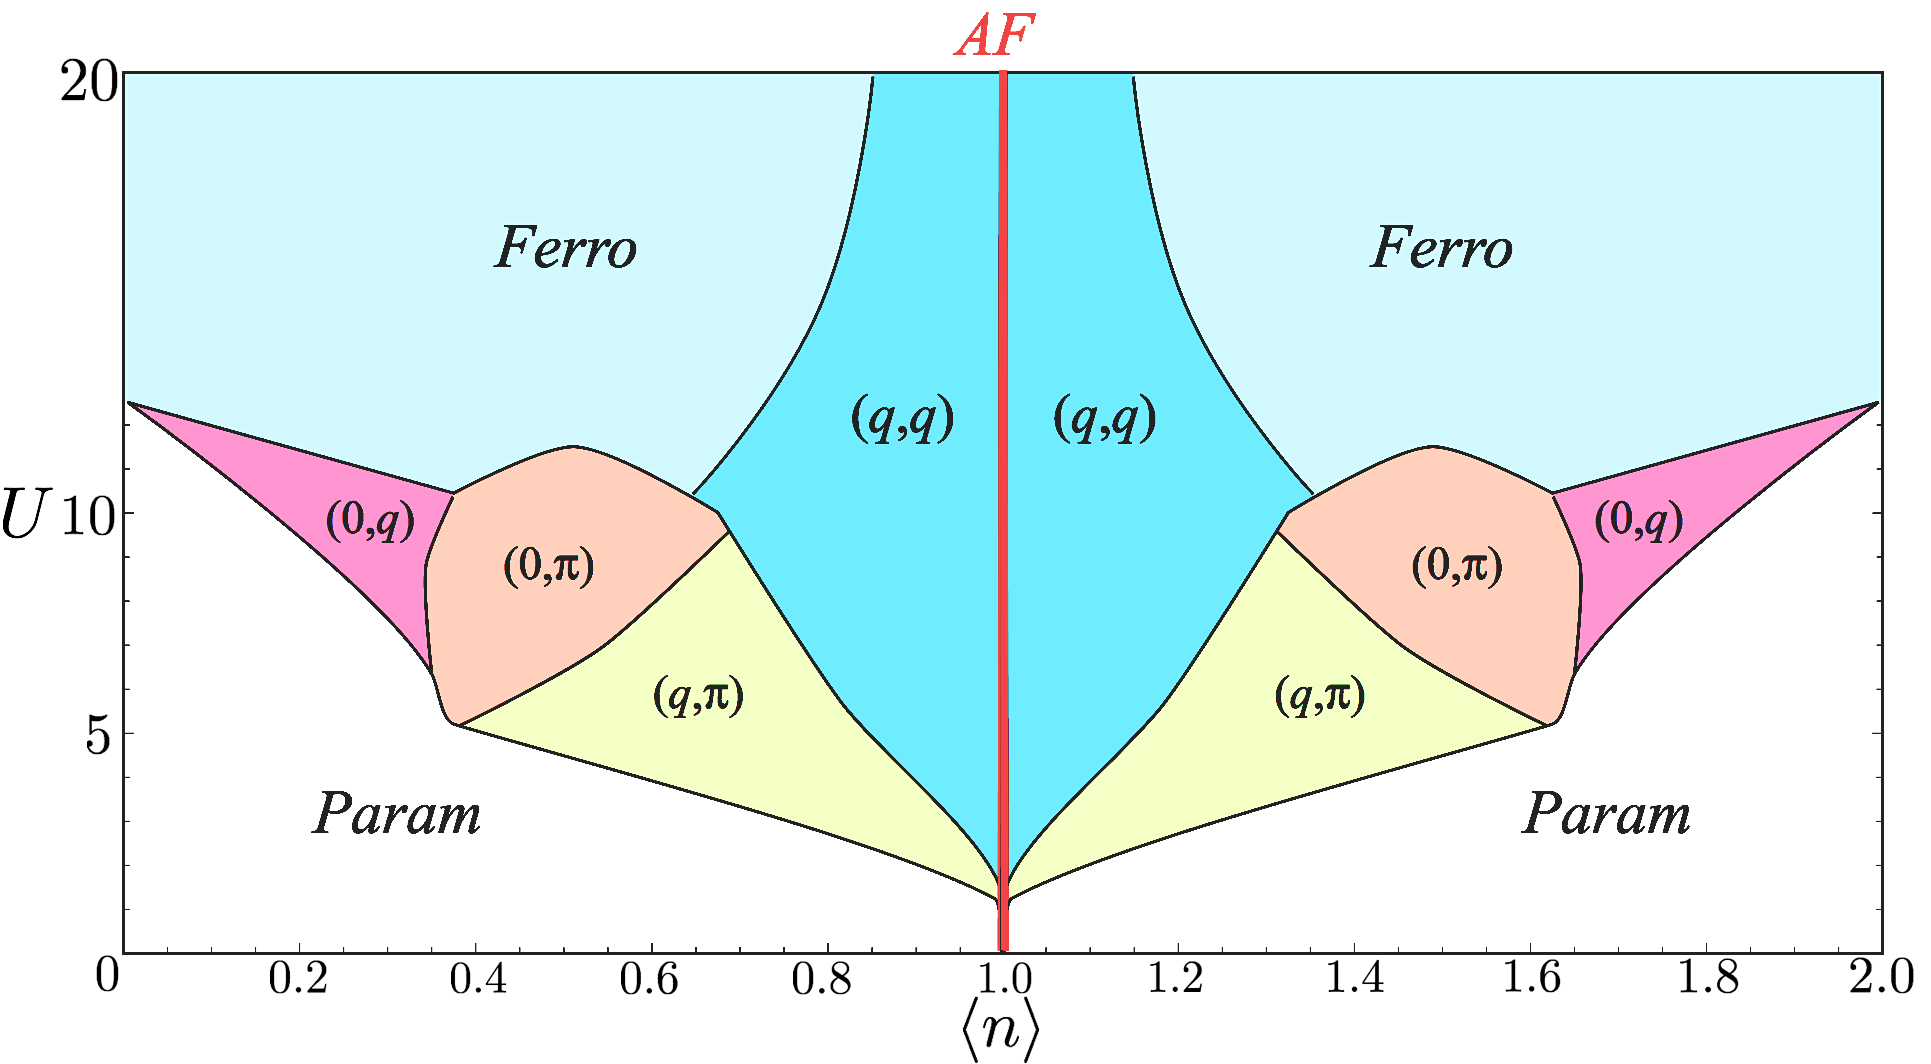
\includegraphics[scale=0.24]{Applications/mf-phase-diagram-hubbard}
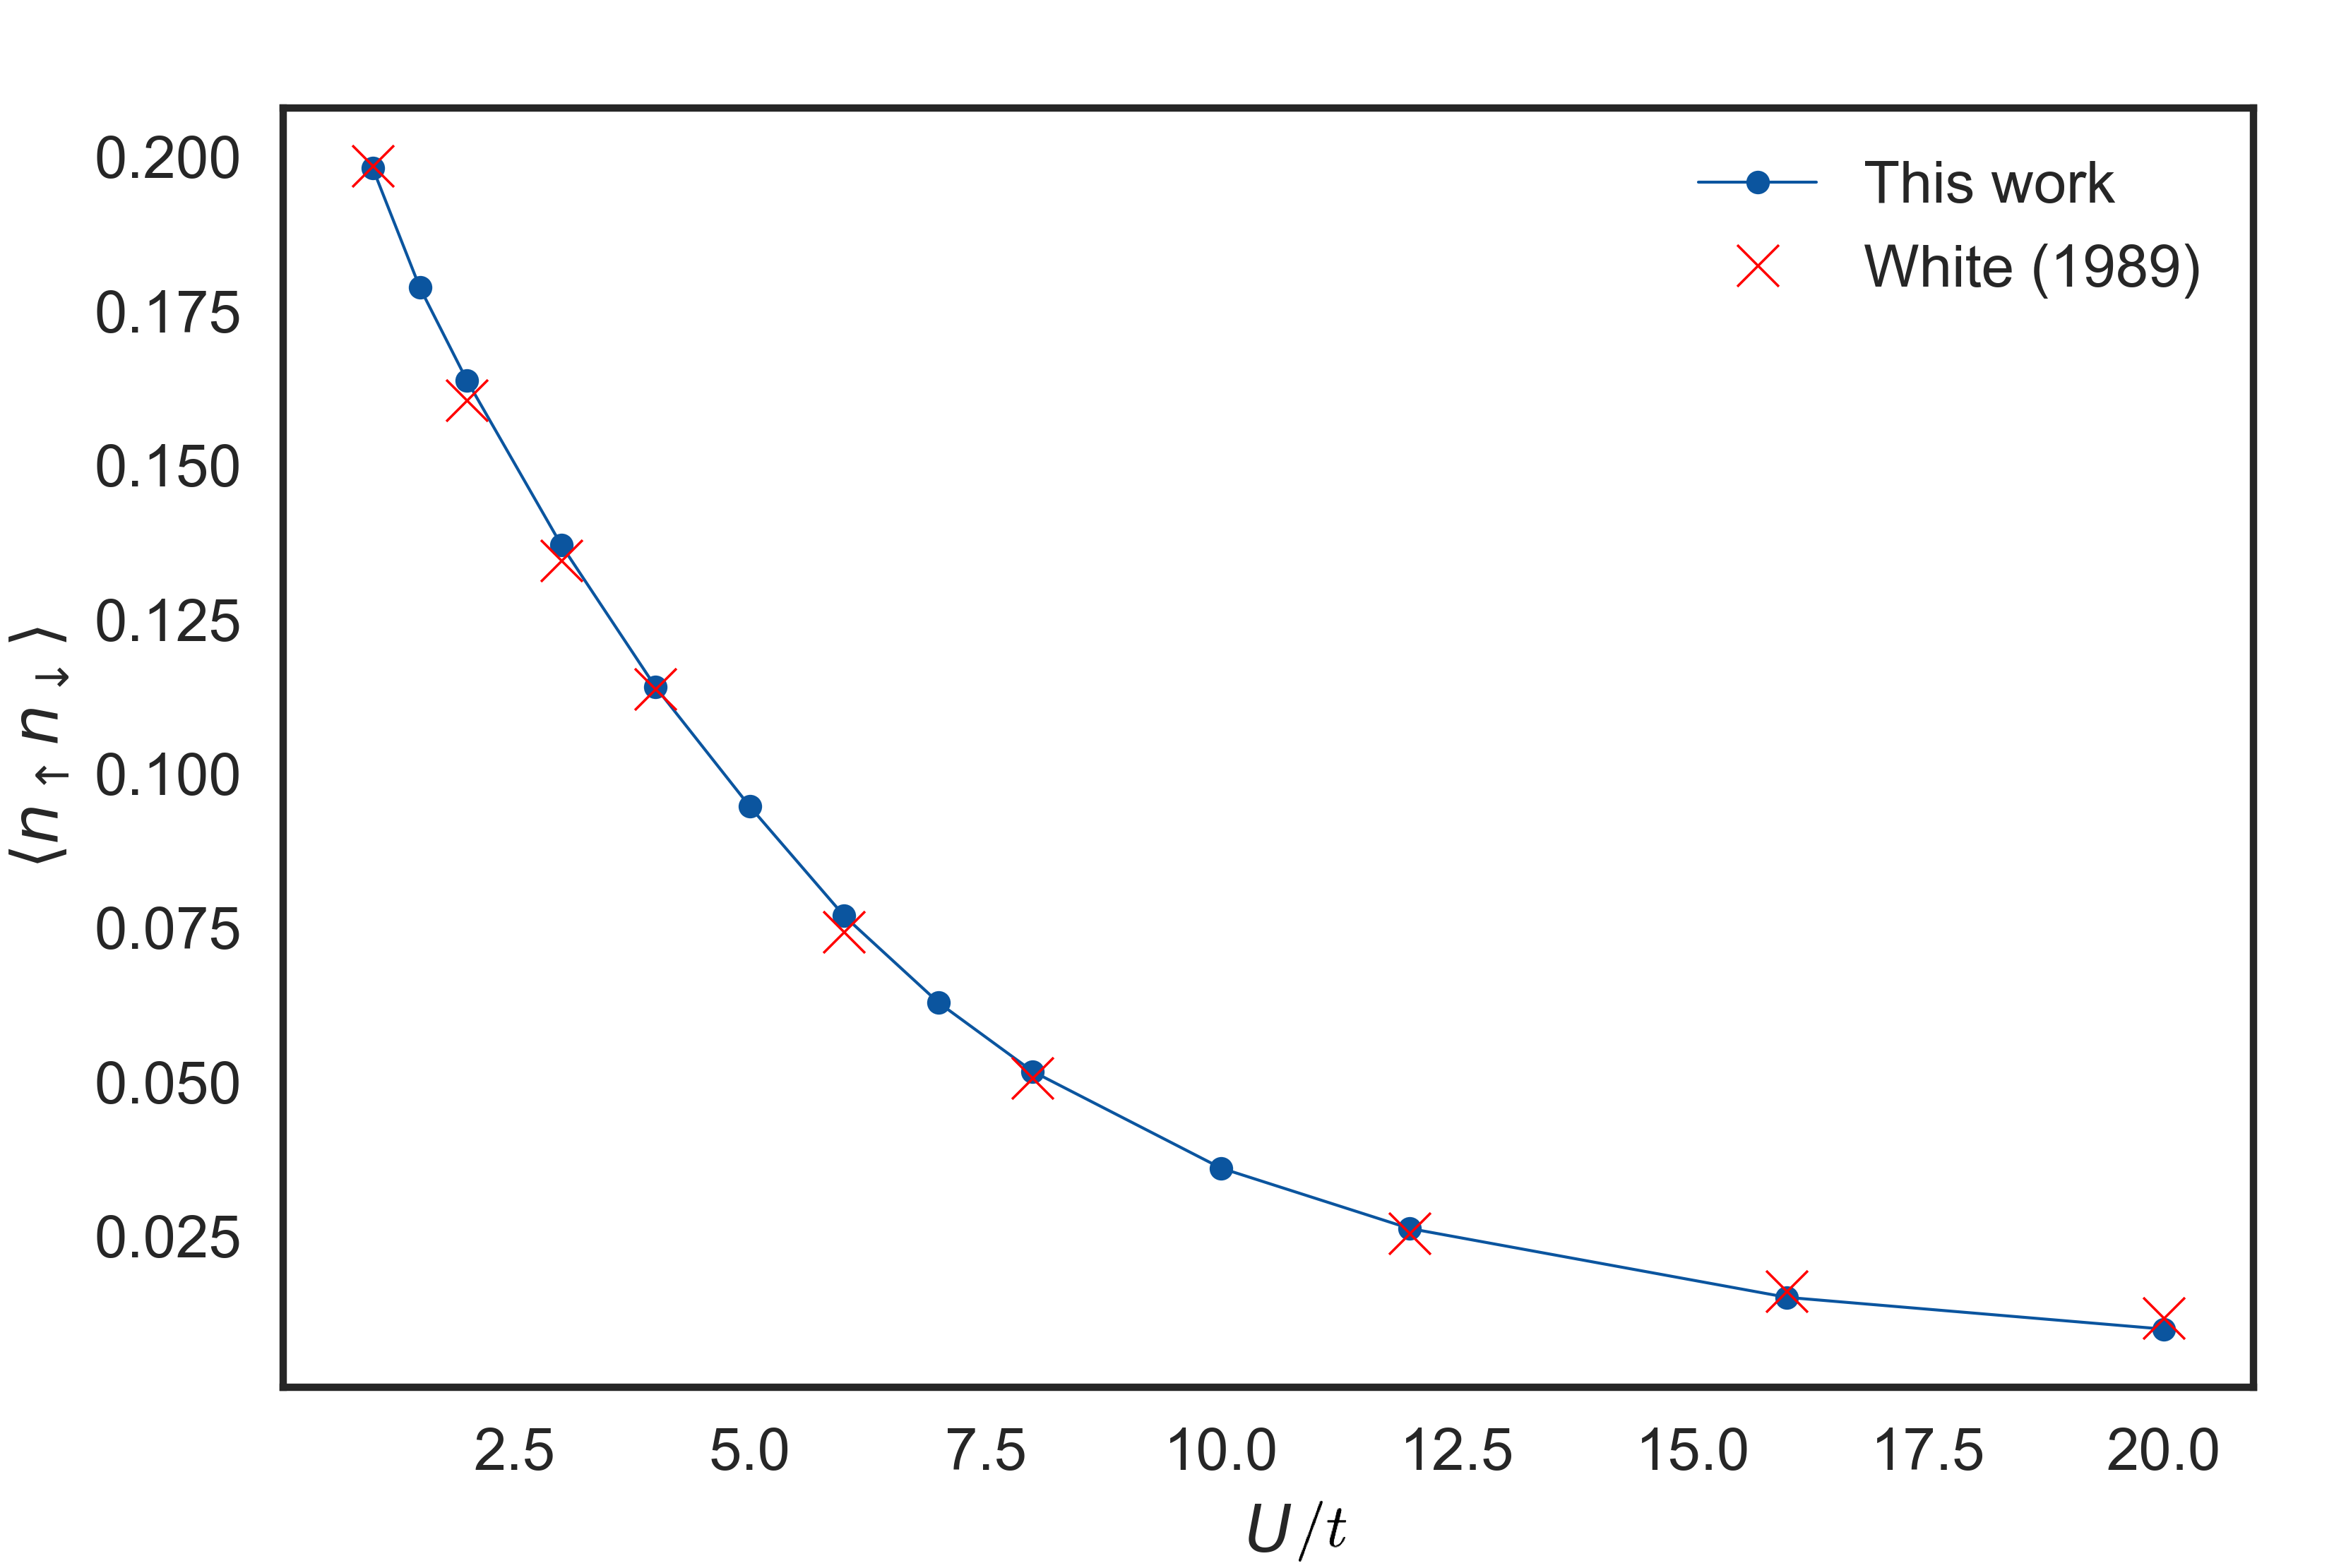
\includegraphics[scale=0.485]{Applications/square/nUpnDwSquare}
\caption[]{\cite{gouveia_magnetic_2015}}
\end{figure}

\begin{figure}[H]\label{fig:corrSq}
\hspace{0.68cm}
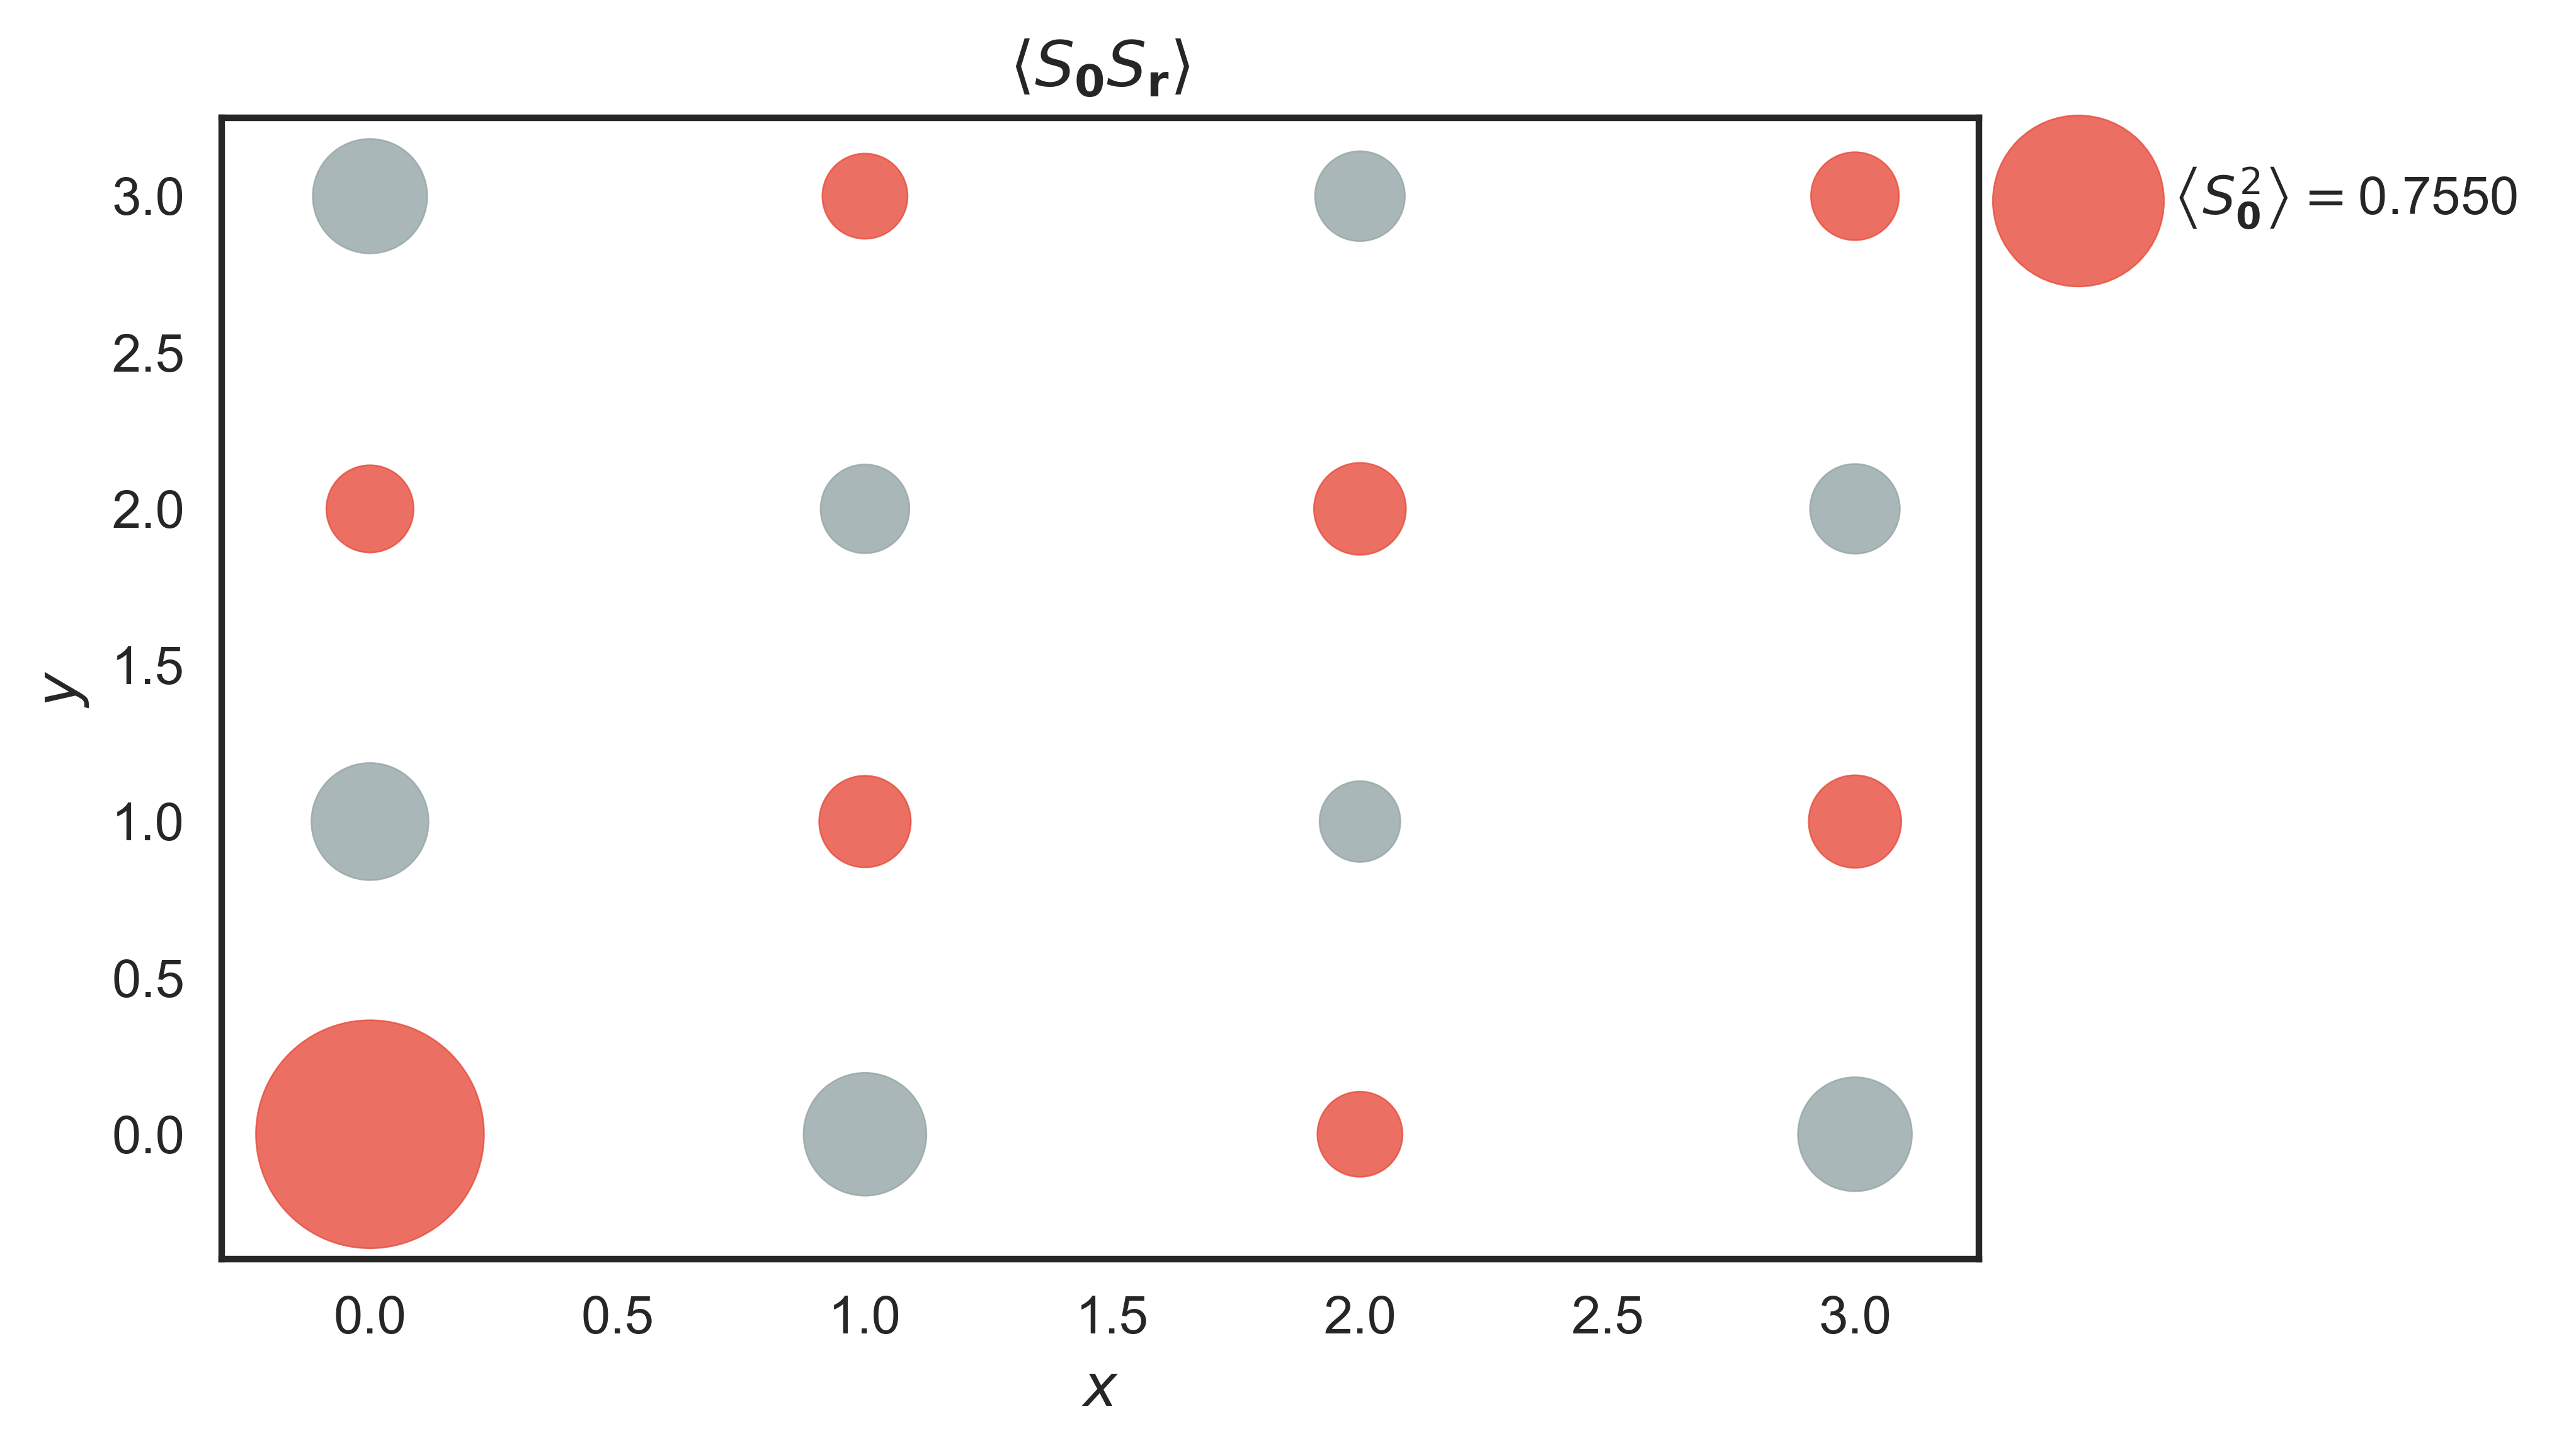
\includegraphics[scale=0.5]{Applications/square/CorrelationsDots}
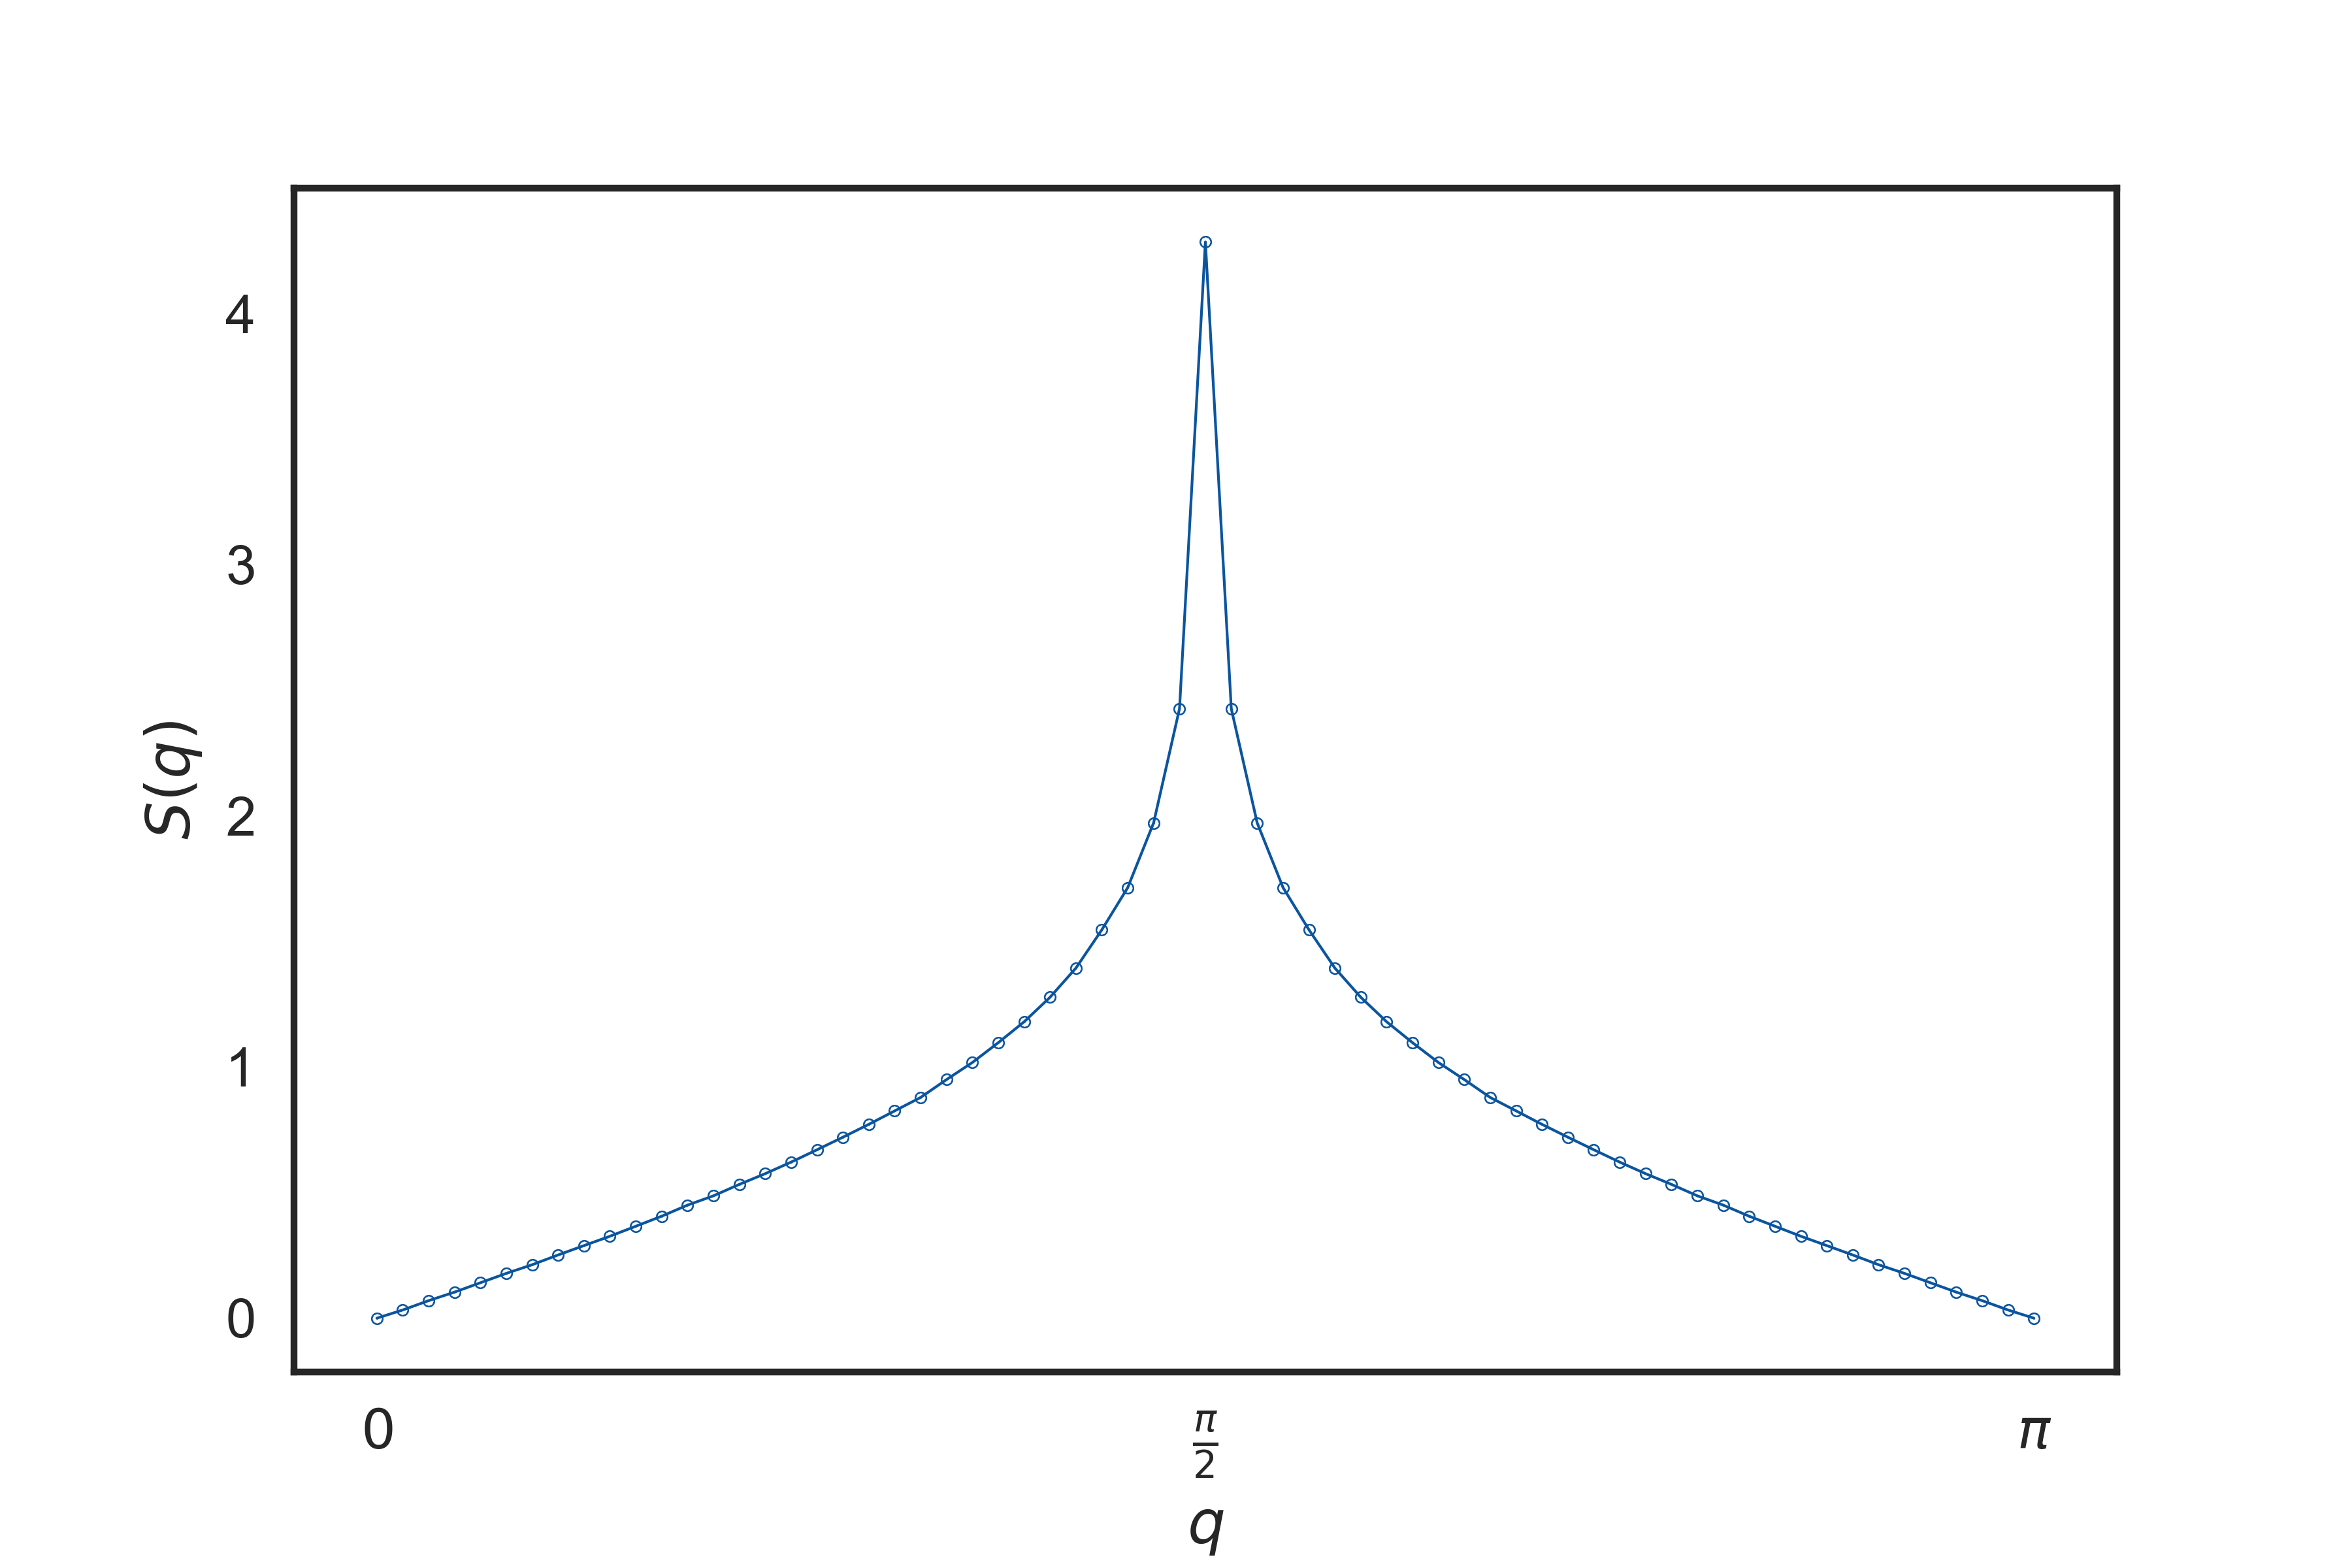
\includegraphics[scale=0.6]{Applications/square/S(q)}
\caption[]{}
\end{figure}

\begin{figure}[H]\label{fig:corrSq}
\hspace{0.6cm}
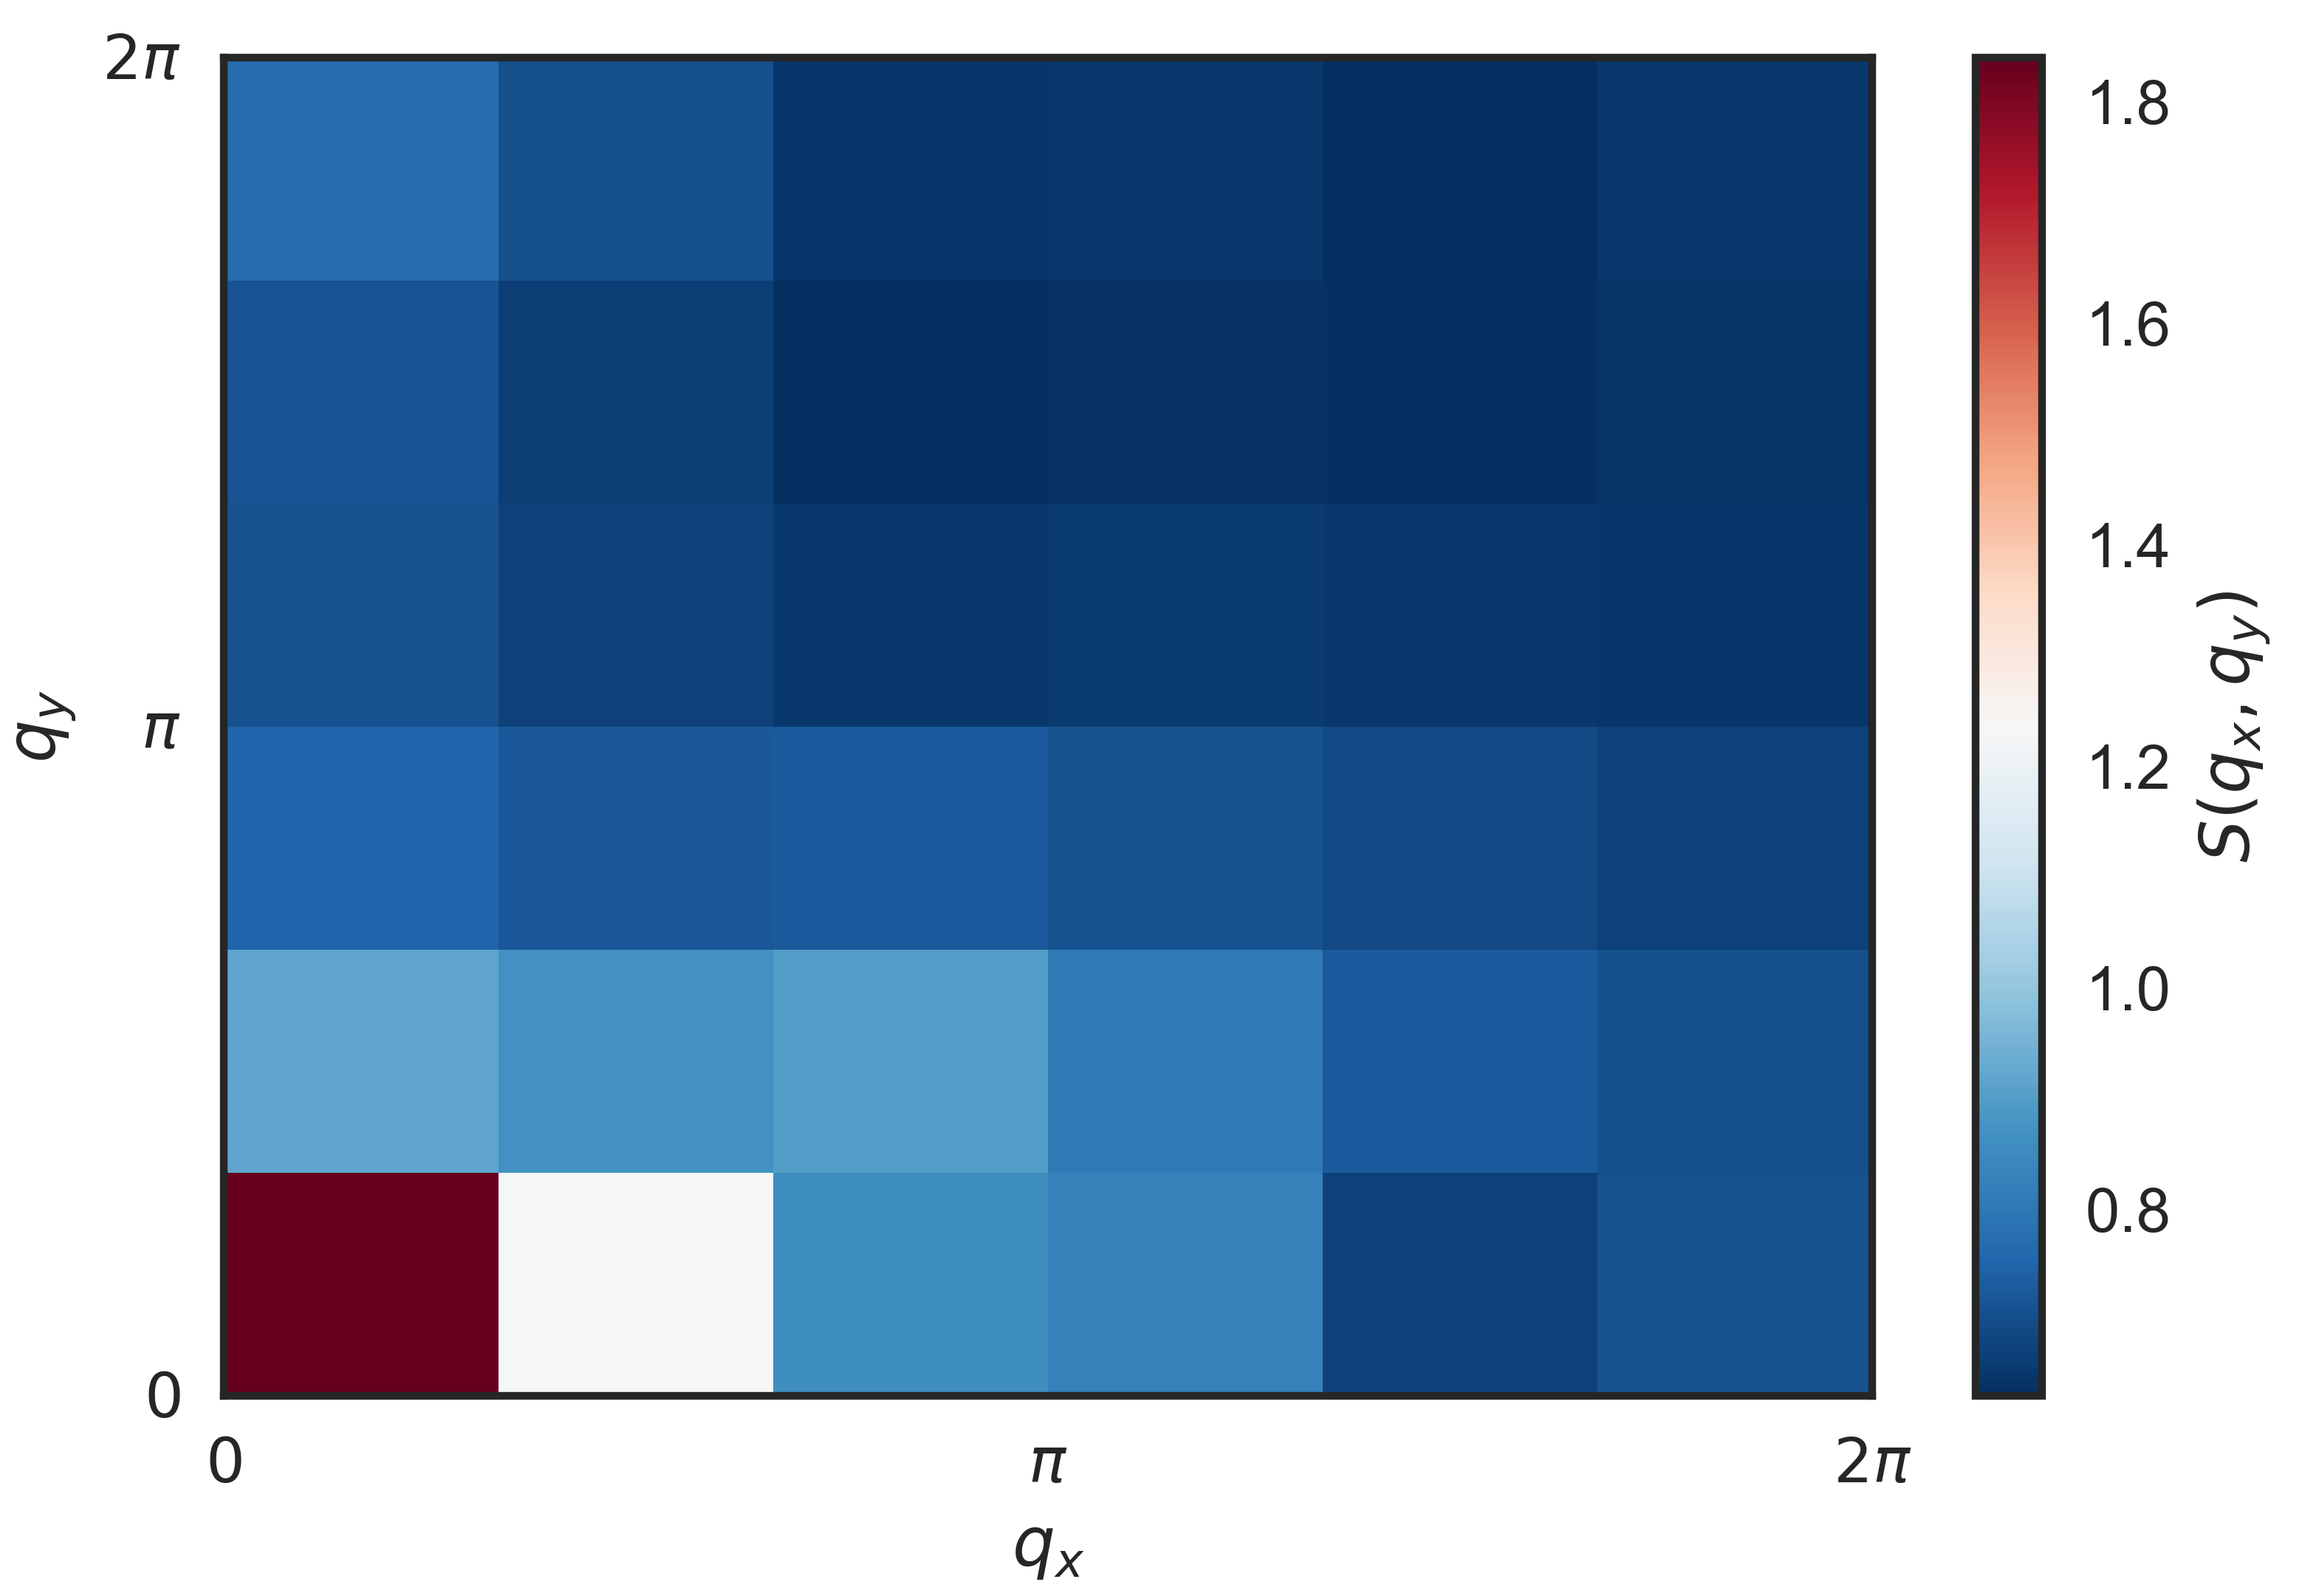
\includegraphics[scale=0.55]{Applications/square/S(q)pcolor.png}
\hspace{1cm}
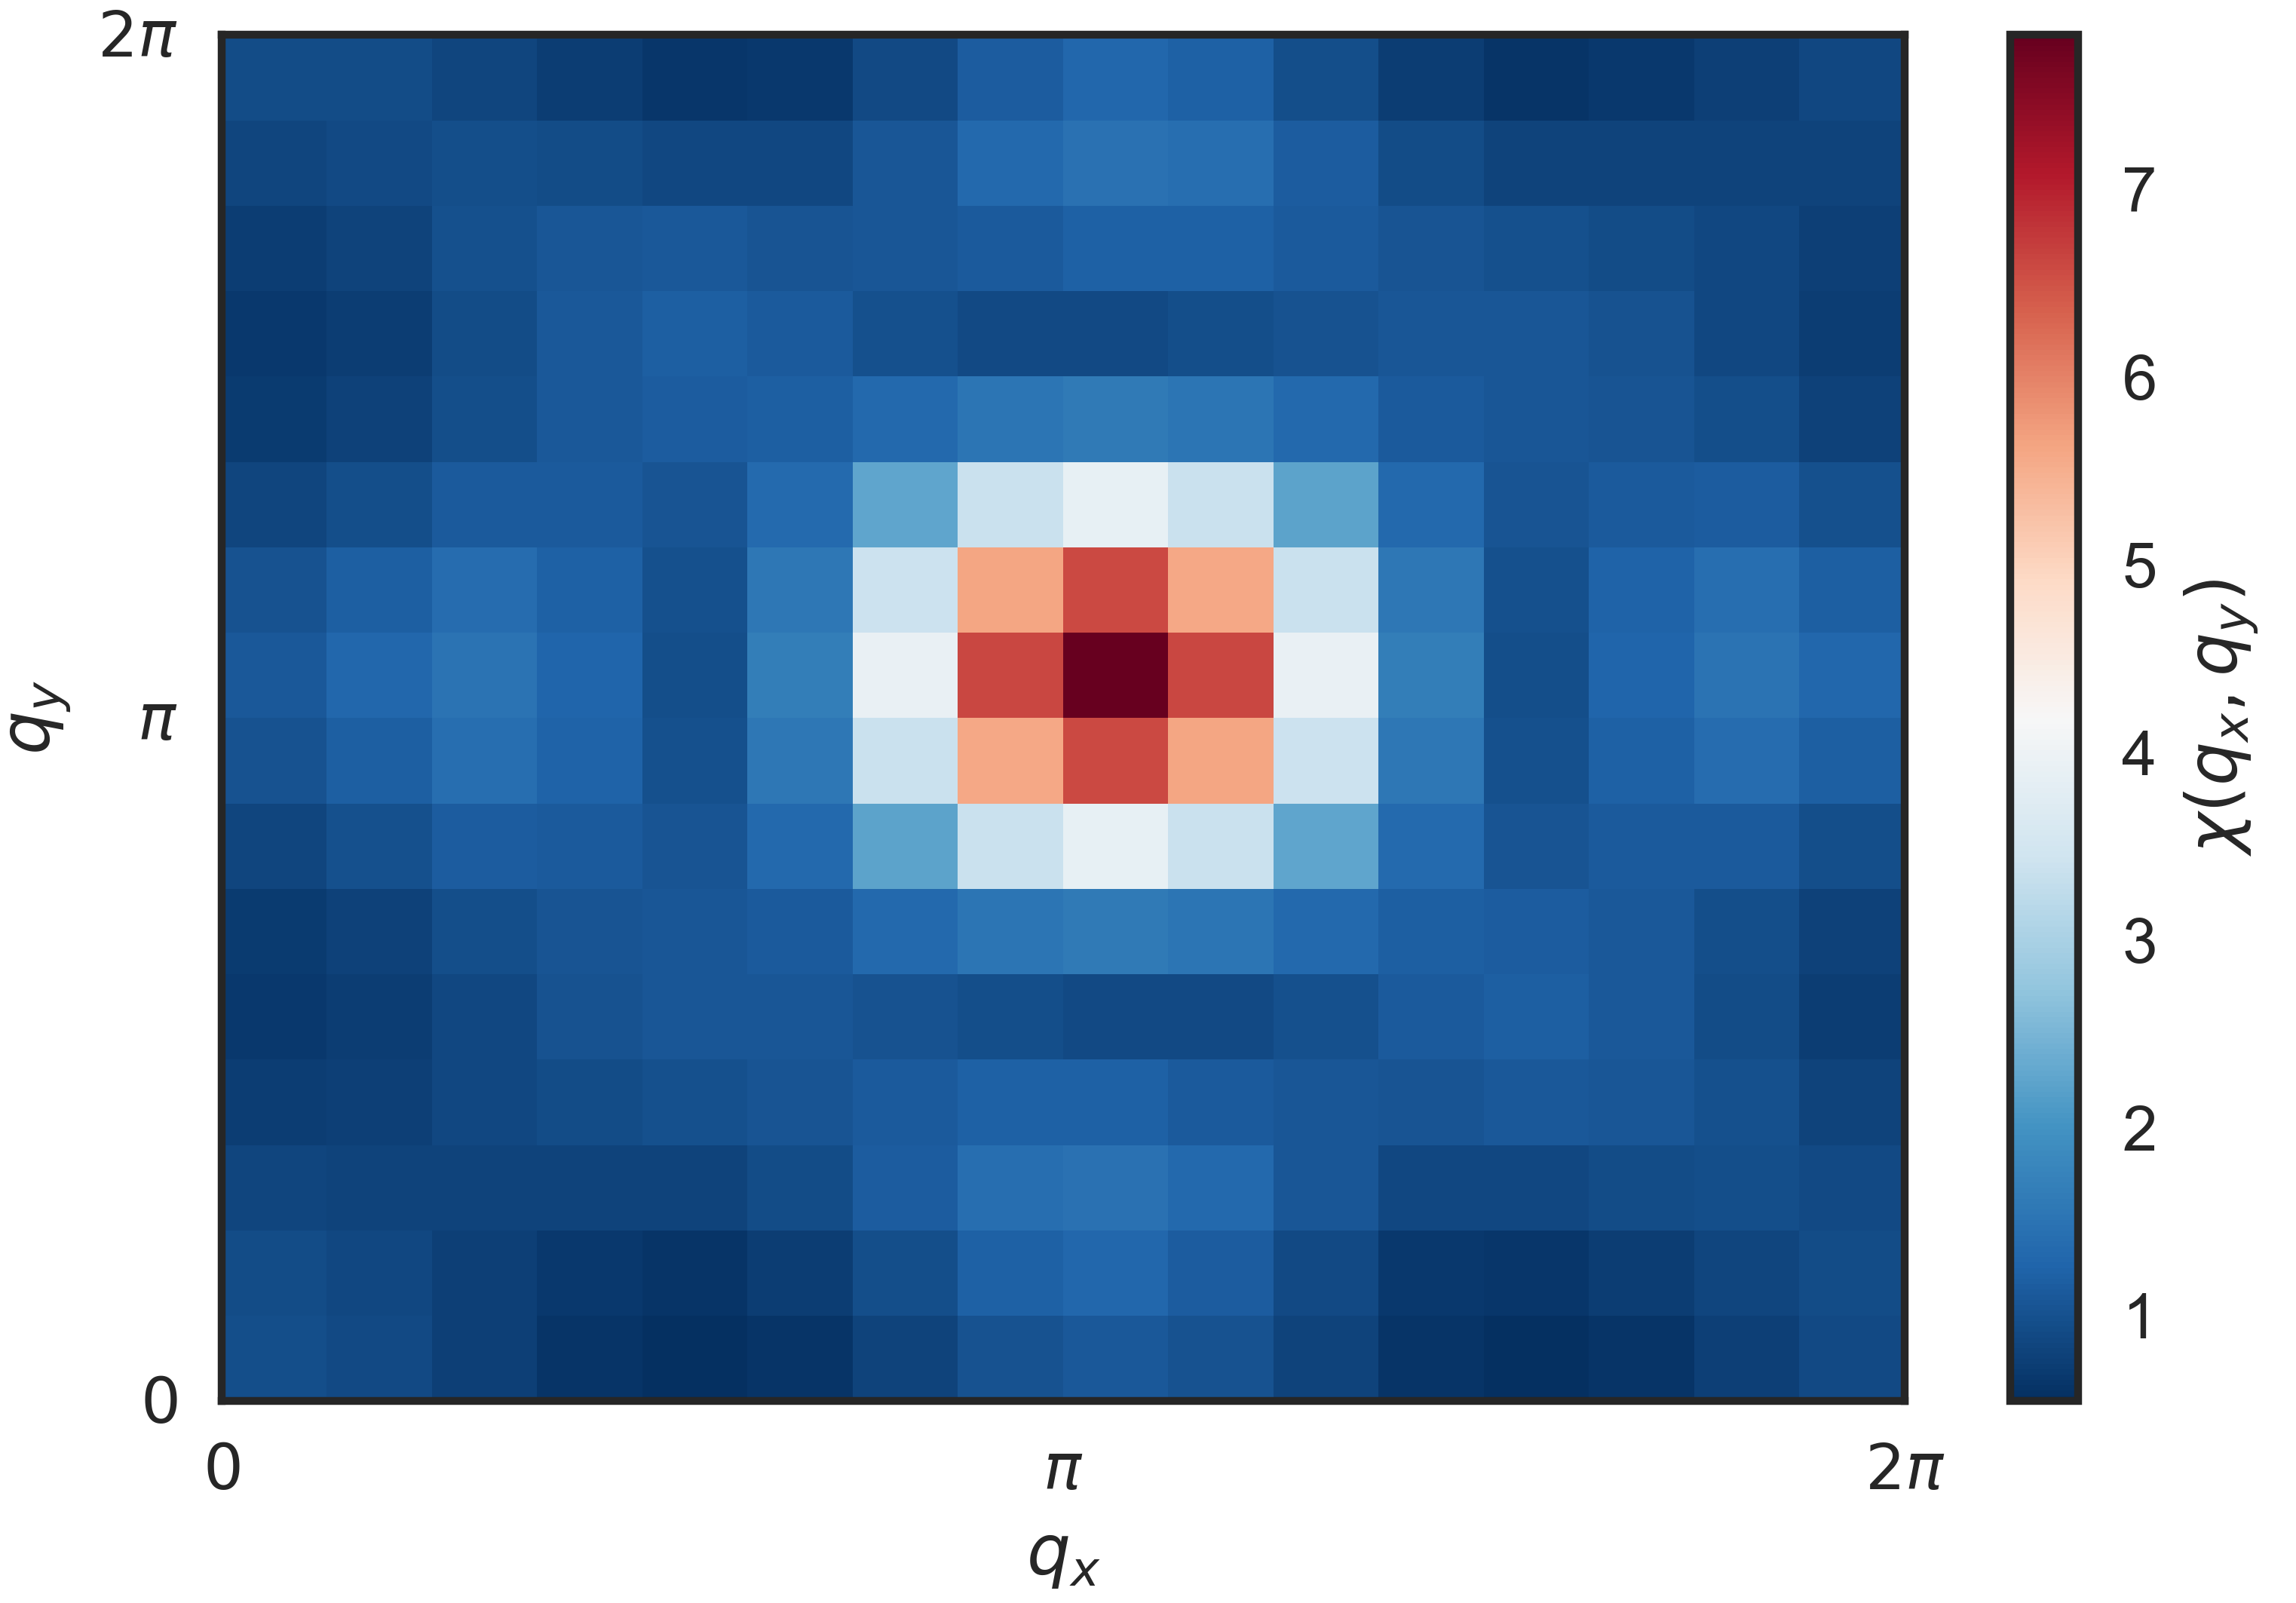
\includegraphics[scale=0.55]{Applications/square/chi(q)pcolor.png}
\caption[]{}
\end{figure}

\begin{figure}[H]\label{fig:corrSq}
\hspace{0.5cm}
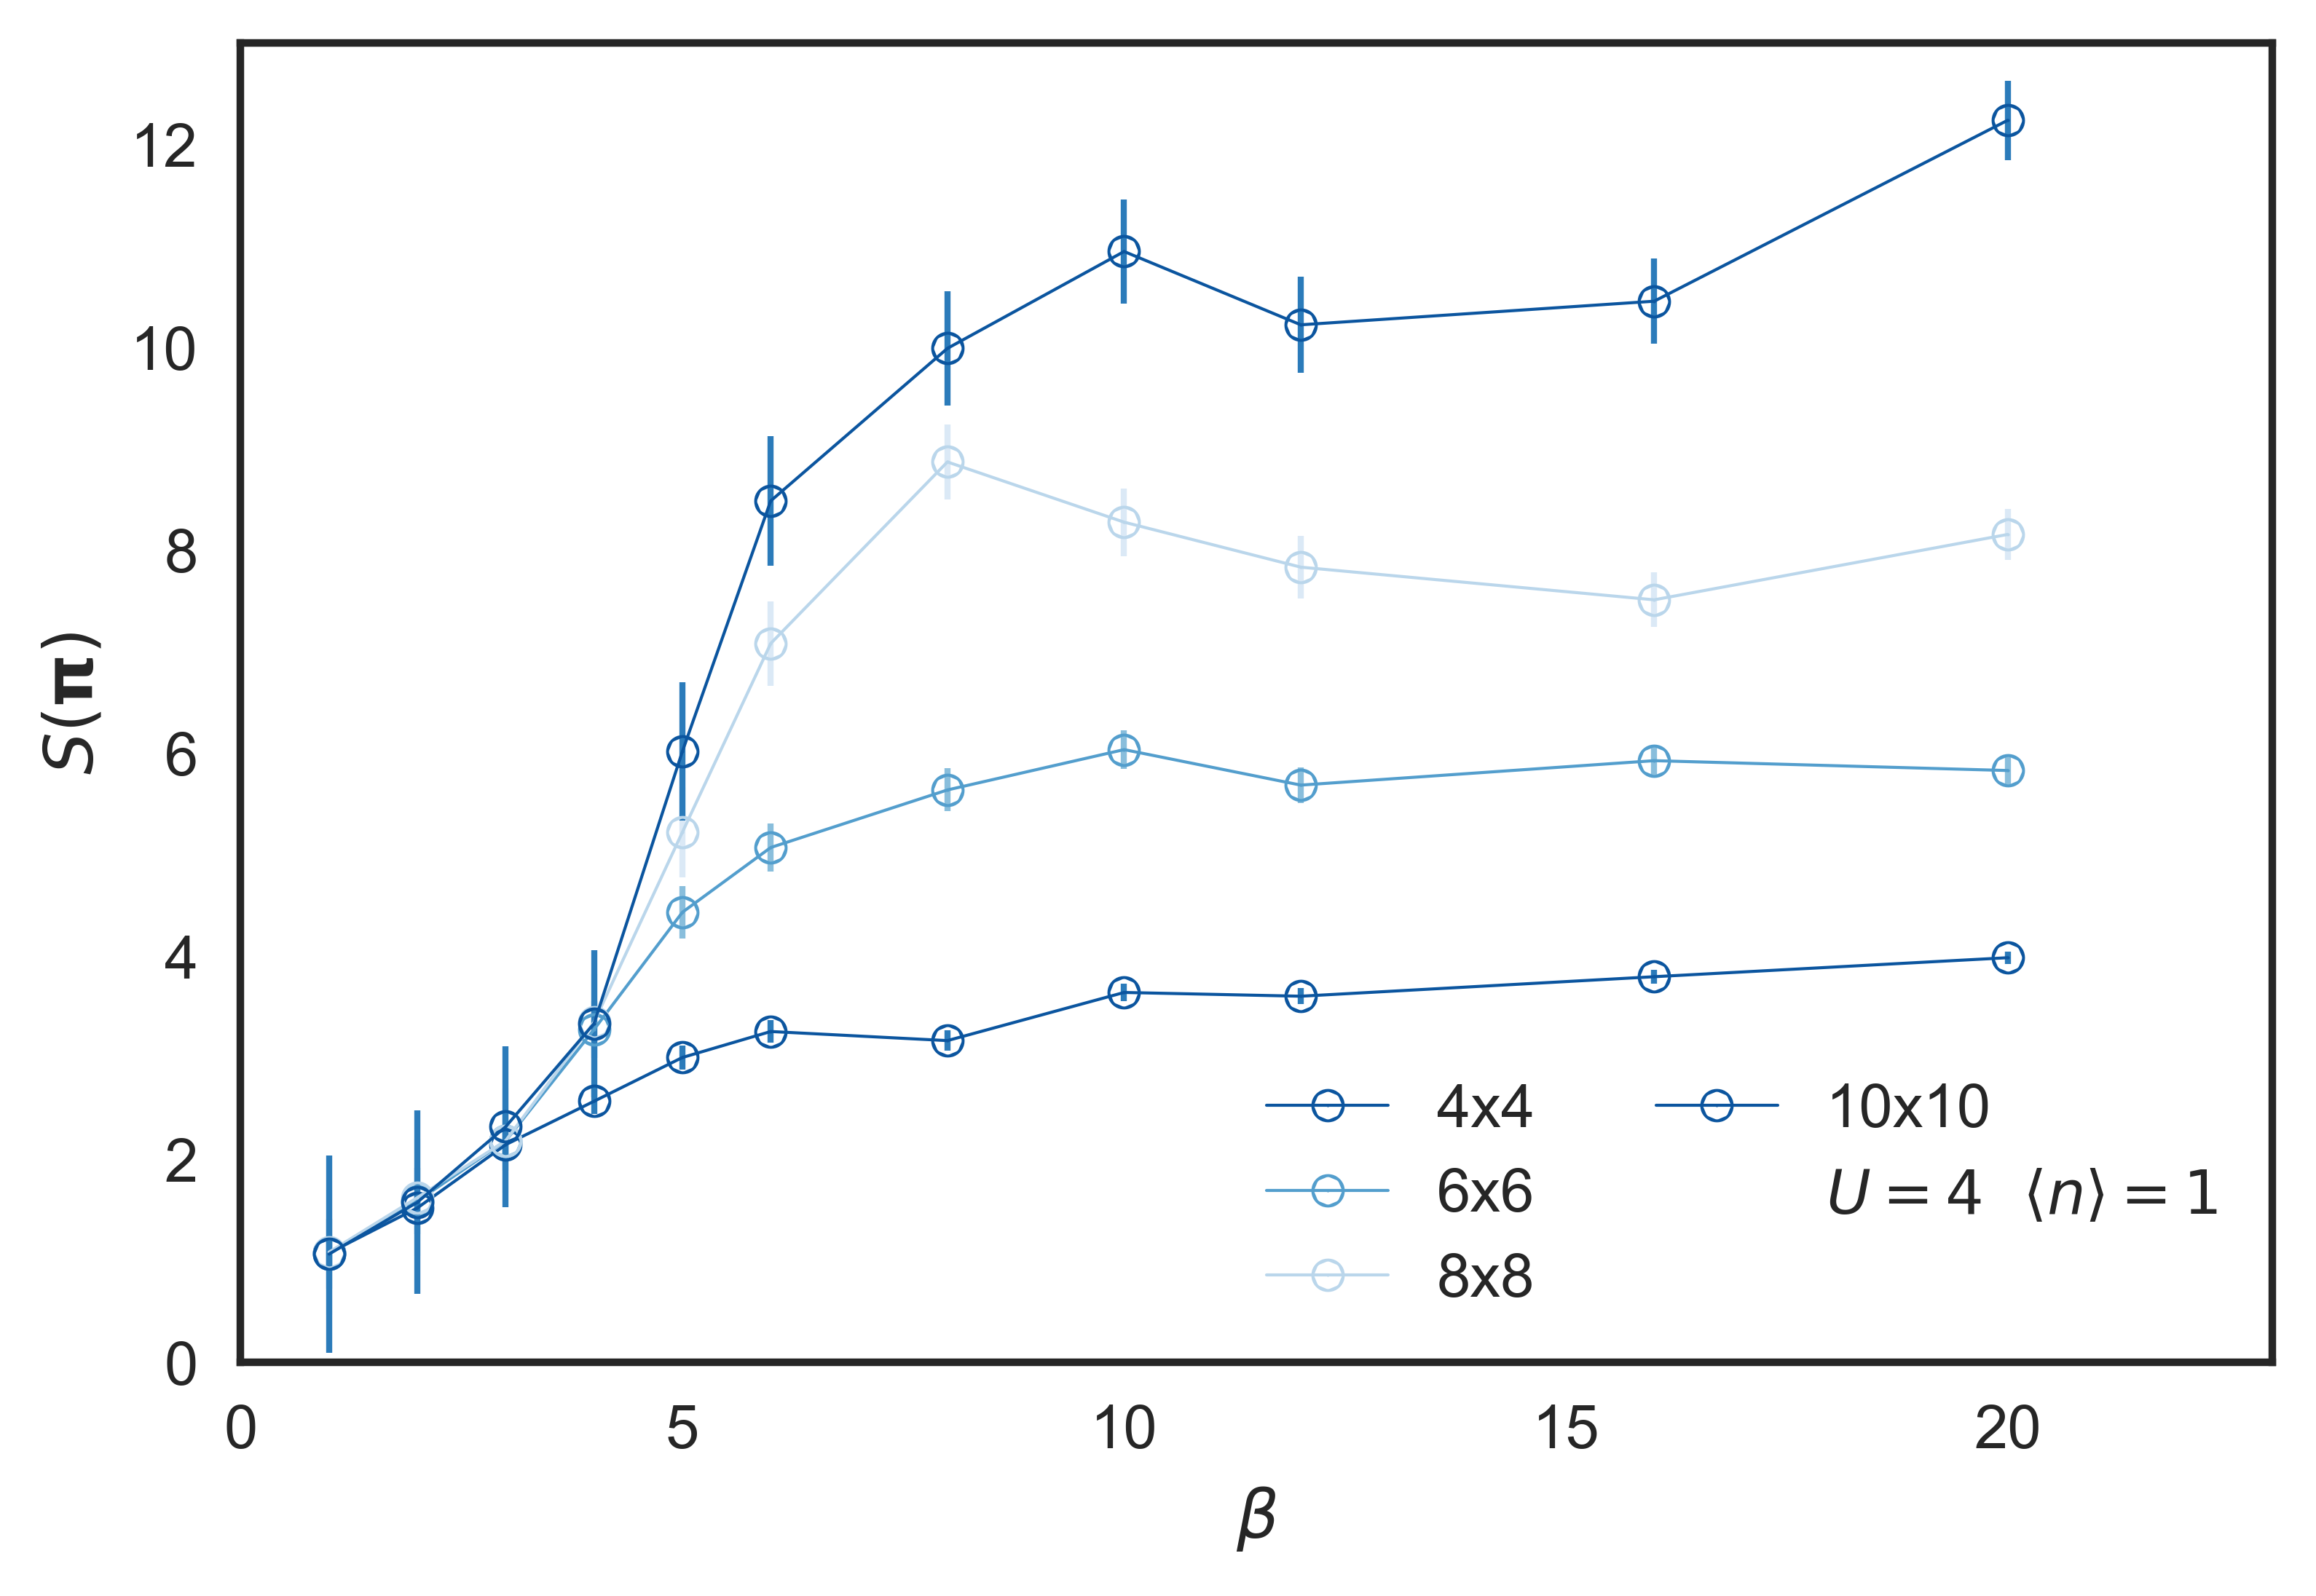
\includegraphics[scale=0.55]{Applications/square/Spipi.png}
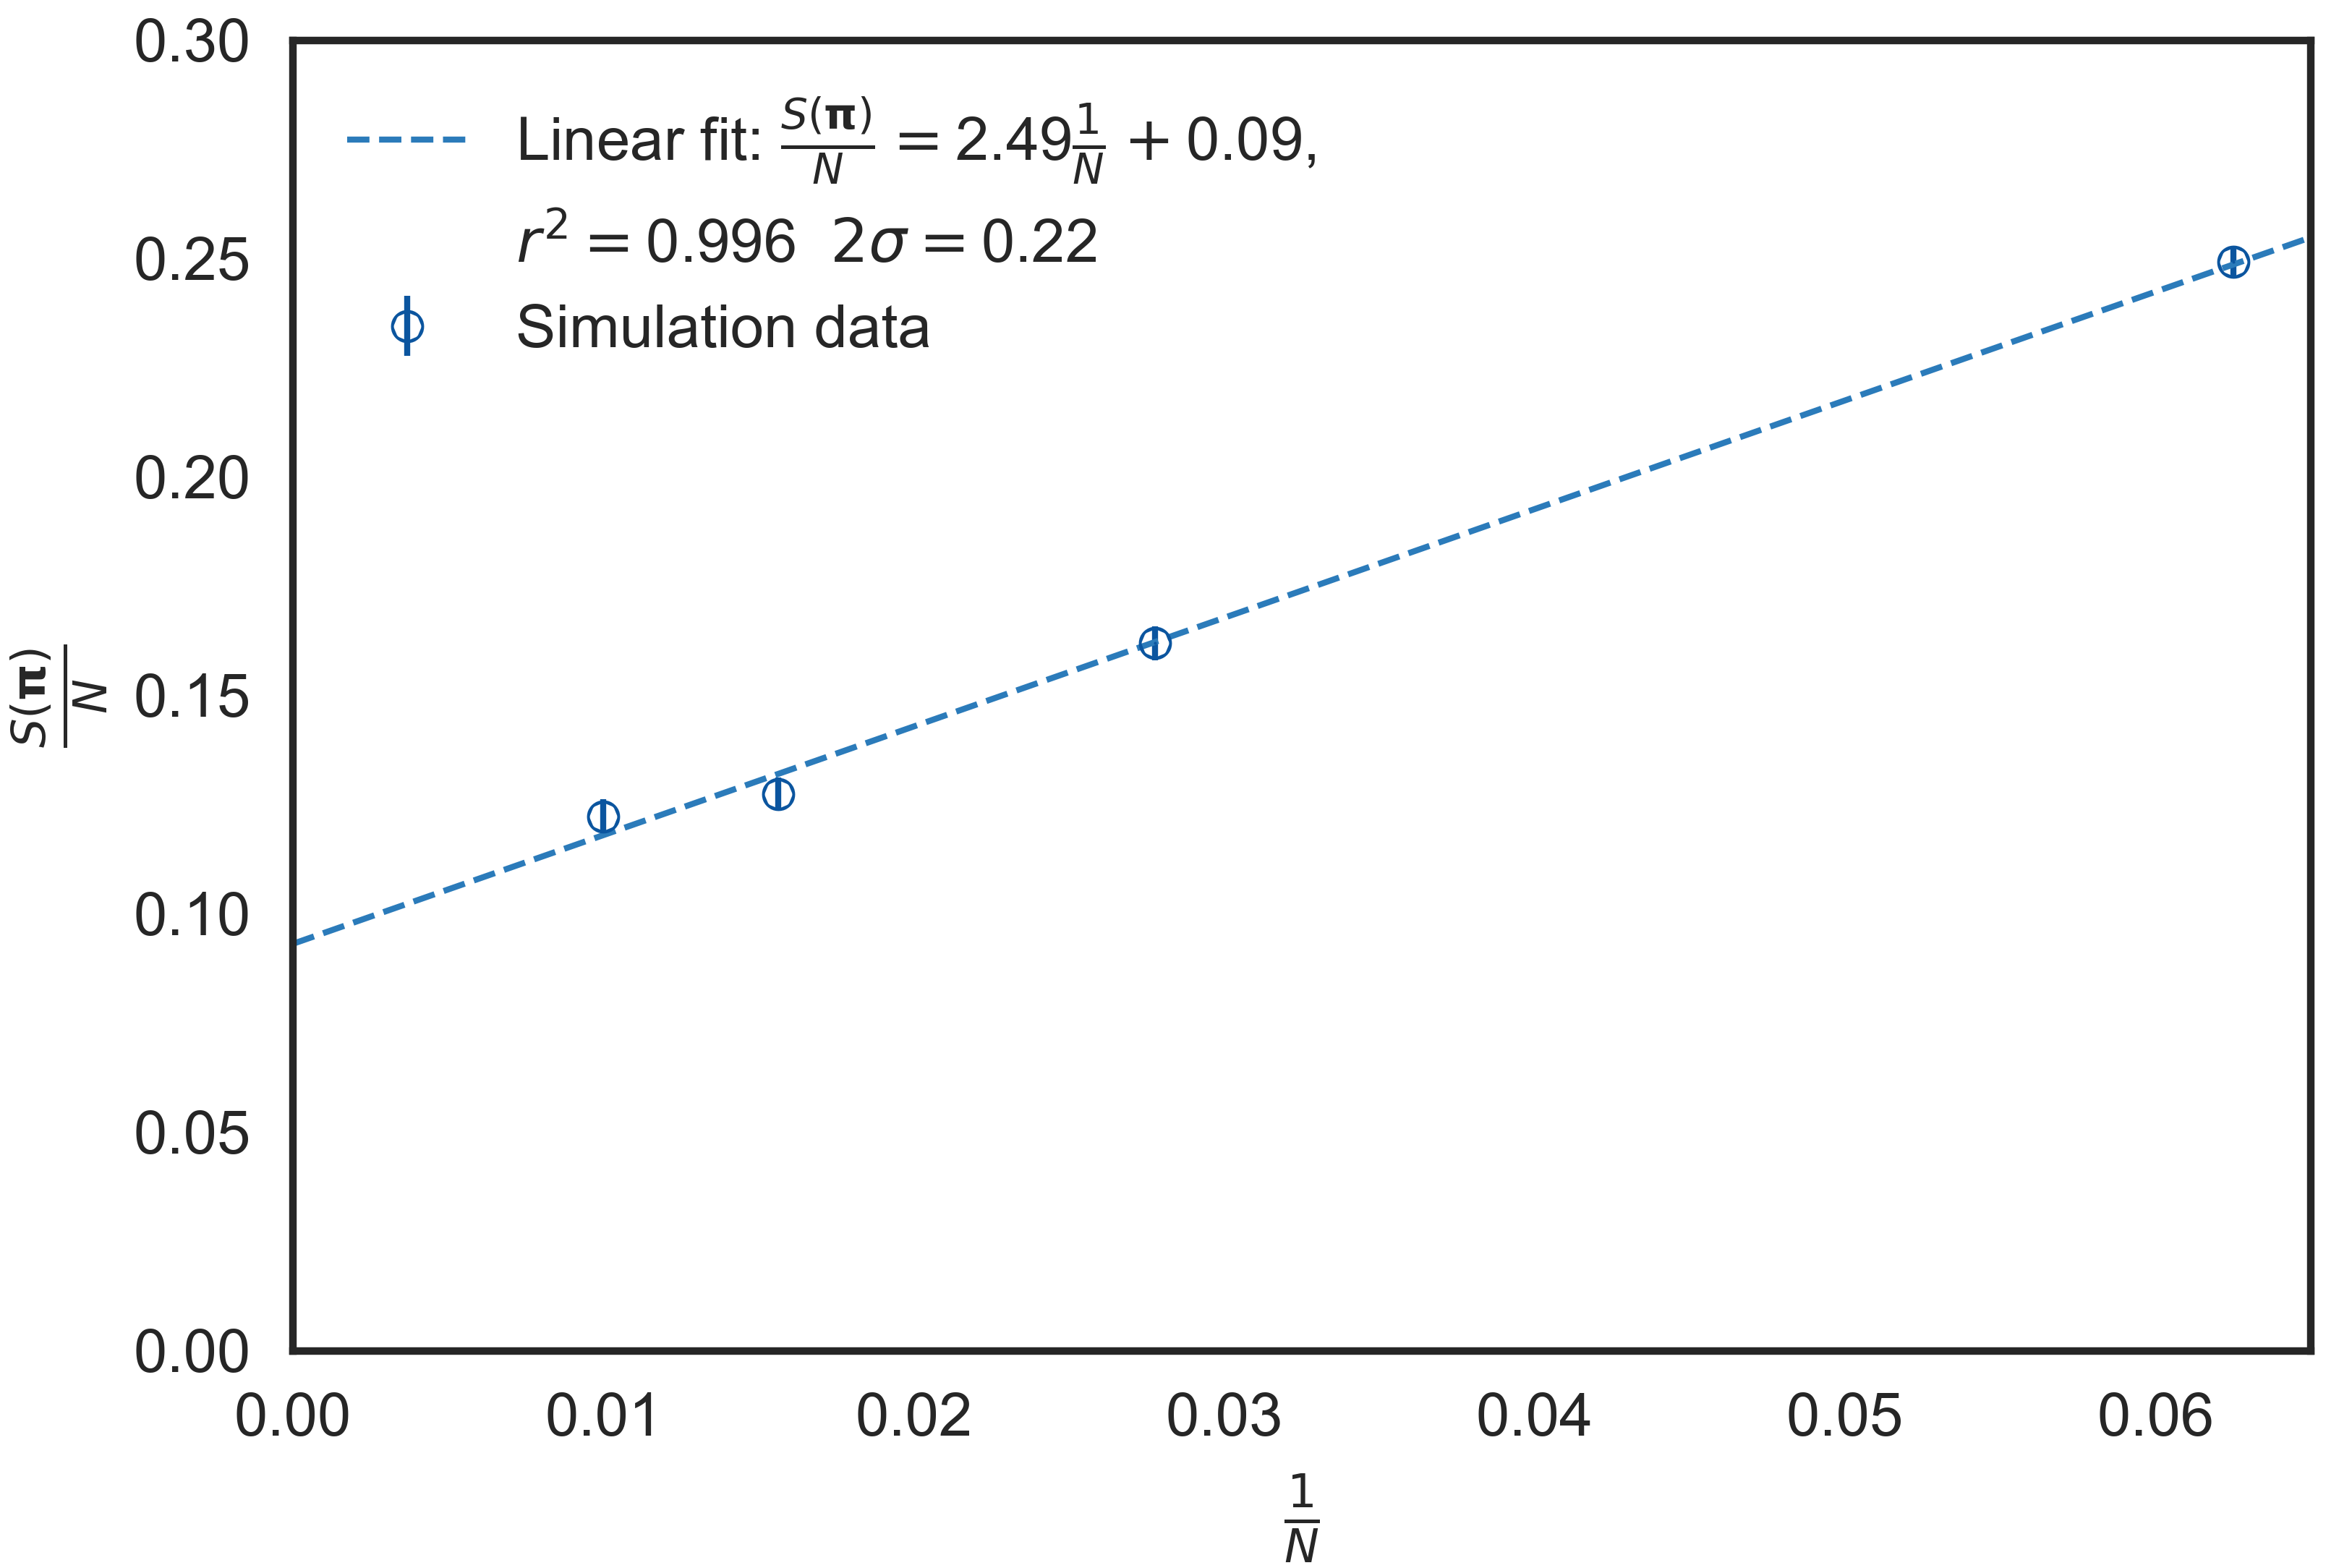
\includegraphics[scale=0.55]{Applications/square/extrapolationSpi.png}
\caption[]{}
\end{figure}